\appendix %% Start the appendices.
\chapter{An appendix}

\section{Time series metrics comparison on UCR datasets}
\label{sec:app-ucr}
Here you can insert the appendices of your thesis.


\begin{table}[htp]
\begin{tabular}{l|r}
\textbf{Distance measure} & \multicolumn{1}{l}{\textbf{Average rank}} \\ \hline
dd\_fdtw\_0.8             & 6                                         \\
dd\_fdtw\_0.6             & 7                                         \\
dd\_sakoe\_chiba\_0.8     & 7                                         \\
dd\_sakoe\_chiba\_0.6     & 7.75                                      \\
dd\_fdtw\_0.4             & 8                                         \\
dd\_itakura\_0.8          & 8                                         \\
dd\_sakoe\_chiba\_0.4     & 8                                         \\
sakoe\_chiba              & 8                                         \\
dd\_dtw\_0.4              & 8.5                                       \\
dd\_dtw\_0.8              & 8.5                                       \\
dd\_itakura\_0.6          & 8.5                                       \\
itakura                   & 8.5                                       \\
dd\_dtw\_0.6              & 9                                         \\
dd\_itakura\_0.4          & 9                                         \\
dtw                       & 10.75                                     \\
fdtw                      & 11                                       
\end{tabular}
\end{table}

\begin{figure}[htp]
    \centering
    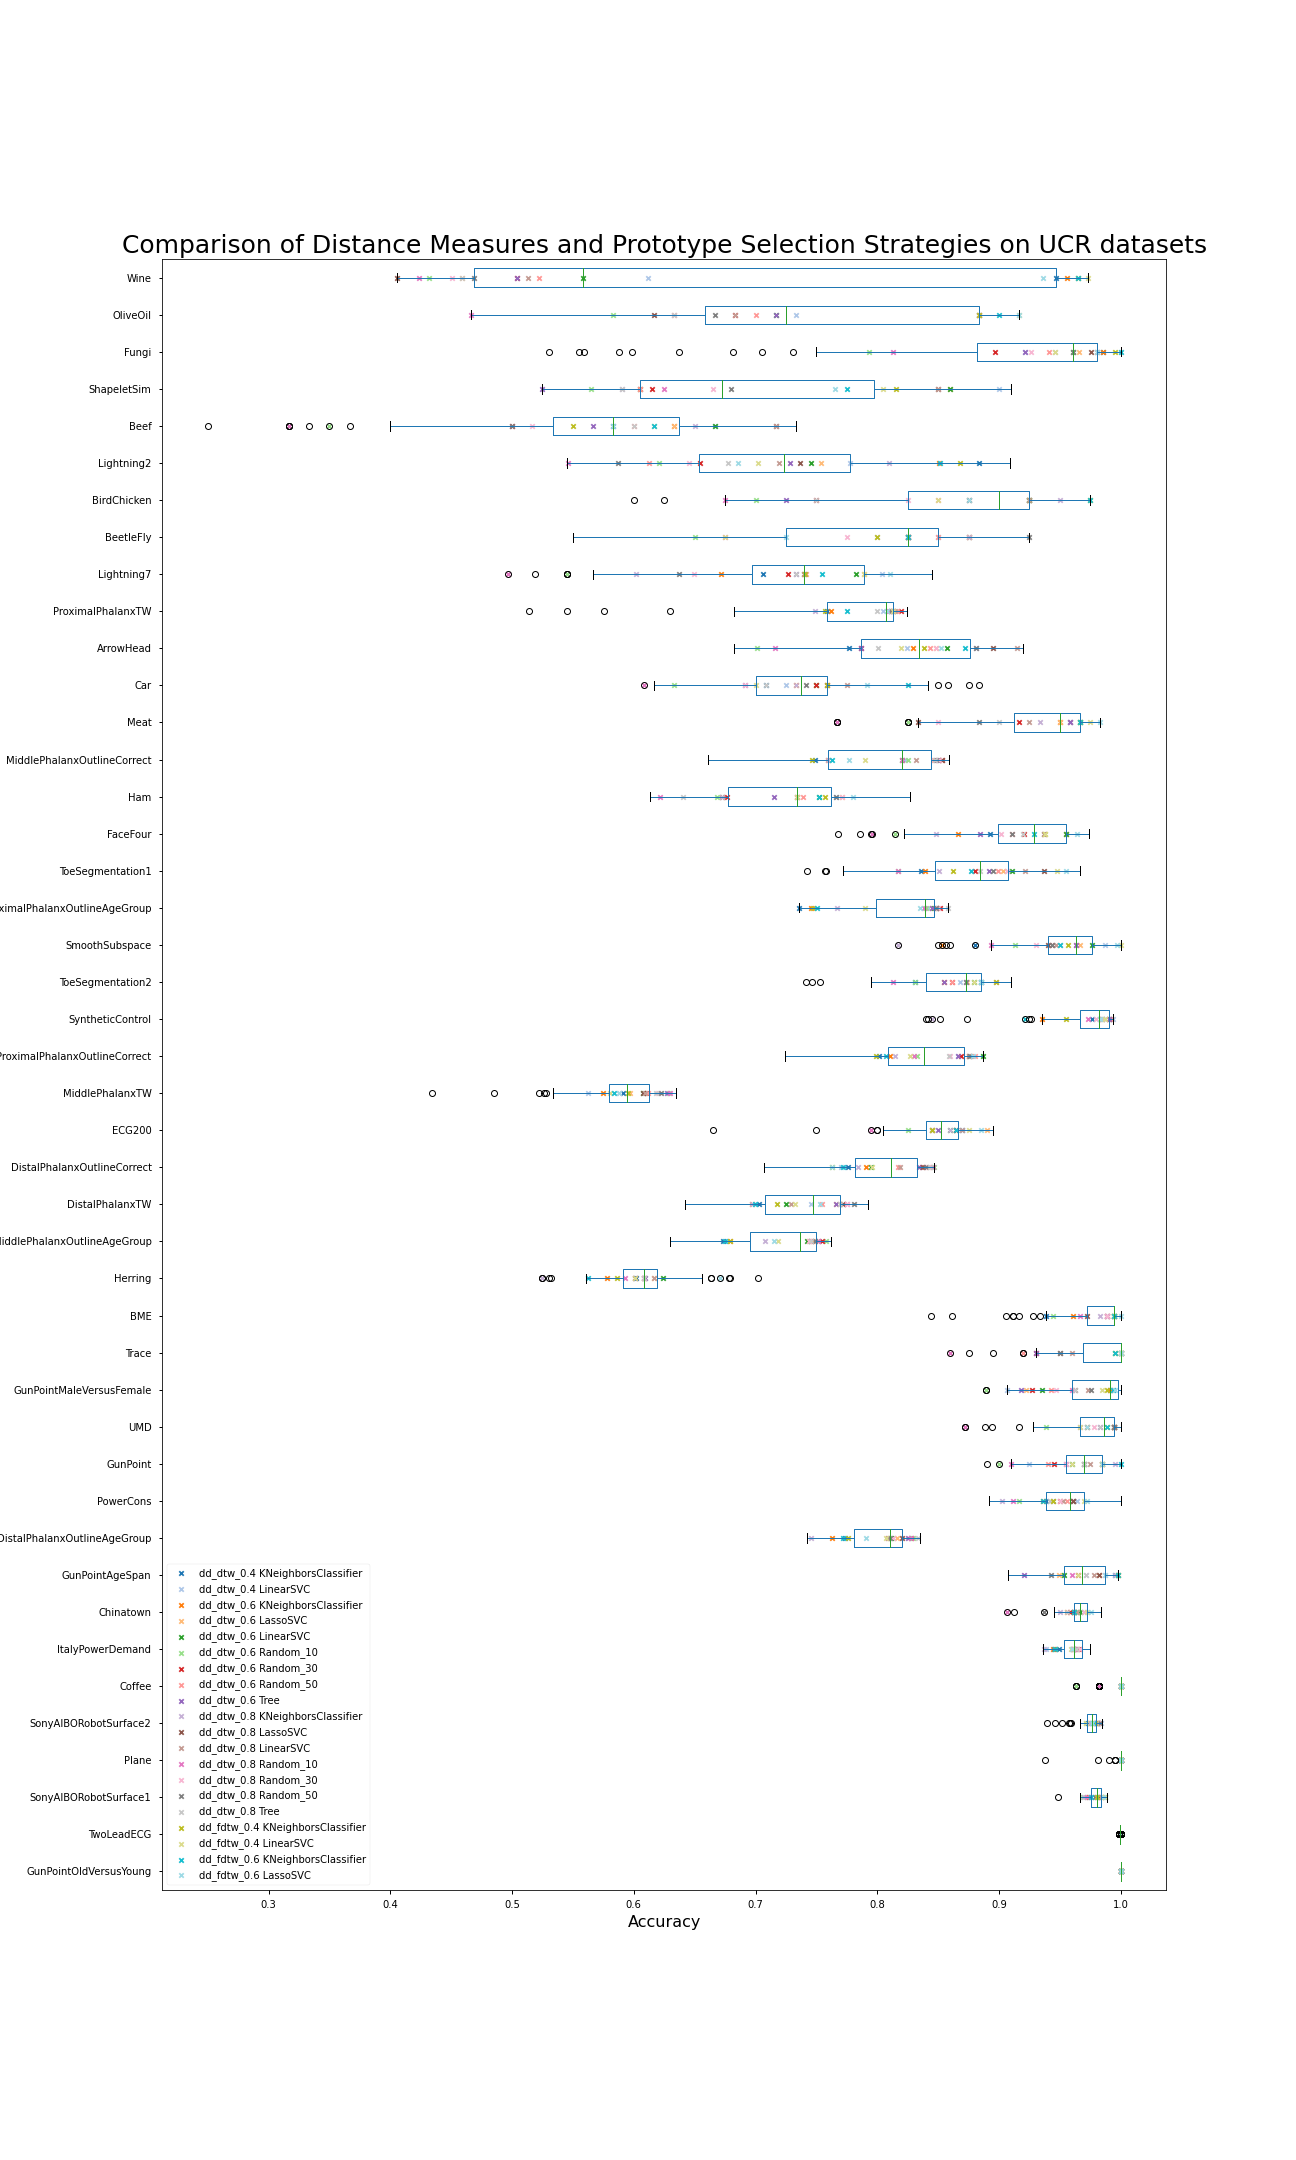
\includegraphics[width=\textwidth]{img/ucr_accuracy.png}
    \caption{TMP}
    % \label{fig:ltob}
\end{figure}


\section{Prototype Selection by Predicting the Correlation Coefficients}
\ref{sec:app-corr}